\chapter{面向FPGA的基于贝叶斯优化的自动化近似乘法器设计方法}


\section{研究背景与现状}

在FPGA中,算术操作通常由DSP模块实现,但DSP电路的面积只占整个FPGA芯片的5\%,且位置固定\cite{FPGA:DSP},这意味着某些需要大量乘法的应用比如DNN无法在FPGA上被有效的映射\cite{FPGA:Math}。相对应的,FPGA中存在着丰富的查找表单元,能够和布线资源一起实现复杂的函数功能,某些充分考虑LUT特性的设计能够在FPGA上实现相当高的性能\cite{FPGA:PolyLUT}。
然而,一块FPGA芯片的容量是有限的,对于大型设计来讲往往需要将其划分后部署到不同的FPGA芯片上,这会极大地降低电路的性能。同时FPGA中的布线资源昂贵,如果查找表单元使用的过多,有可能会造成布线拥塞,也会对电路的性能造成影响。
所以有必要在FPGA中使用近似乘法器来提高乘法的效率,降低FPGA资源的使用量,提高电路的性能。

目前已有的近似乘法器的工作大多是面向ASIC的\cite{AC:AM:KMap,AC:AM:DRUM,AC:AM:SDLC,AC:AM:Adapt,AC:AM:CGP_Evoapprox8b,AC:AM:OU,AC:AM:CR,AC:AM:AC},由于组合逻辑(Combinational logic)在ASIC中由逻辑门(Logic gate)和金属线(Metal wire)构成而在FPGA中由LUT和布线资源组成,因此基于ASIC实现的近似乘法器在FPGA上往往无法获得相同程度的硬件性能提升,需要专门开发面向FPGA架构的近似乘法器设计方法。

\begin{figure}[!h]
    \centering
    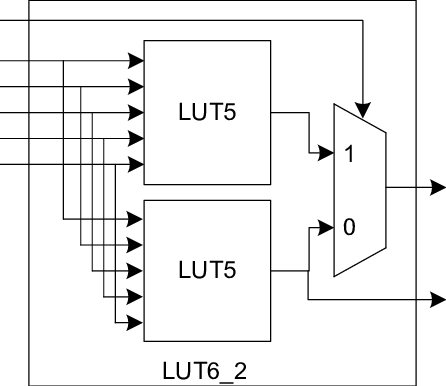
\includegraphics[width=0.5\linewidth]{figs/FPGA-LUT6_2.png}
    \caption{一个典型的拥有6个输入的LUT结构图}
    \label{FPGA:Fig:LUT6_2}
\end{figure}

LUT通常由多路选择器MUX和SRAM构成,其大小可根据输入个数的不同进行区分,一个$n$输入的LUT包含$2^n -1$个MUX和$2^n$个SRAM,能实现任意的$n$输入函数(共$2^{2^n}$个),可看作两个$n-1$的输入LUT和一个二选一MUX的组合。
目前最常用的LUT的输入个数为6\cite{FPGA:VIB},简称为LUT6。图\ref{FPGA:Fig:LUT6_2}展示了一个由两个LUT5组成的LUT6示意图,被称为LUT6\_2。LUT6\_2共包含$64$个SRAM,在编码后每个SRAM都有一个确定的值,被称为初始(Initial, INIT)值,不同INIT值的组合能够实现不同的函数,一共有$2^{64}$种组合,能够实现任意的6输入函数。

\begin{figure}[!h]
    \centering
    
\includegraphics[width=0.4\linewidth]{figs/FPGA-carry_chain.png}
    \caption{一种2比特位宽的FPGA进位链结构示意图}
    \label{FPGA:Fig:carry_chain}
\end{figure}

虽然LUT能够实现特定输入数下的任意单输出函数,但对多输入多输出的算术操作的运算效率并不高。
考虑到加法使用最频繁,为了提高性能,FPGA引入了进位链来降低加法的进位延迟,
一种典型的2比特位宽的进位链结构如图\ref{FPGA:Fig:carry_chain}所示,由两个进位单元级联而成,每个进位单元包含一个LUT和一个伪全加器FA$'$,每个LUT的结构如图\ref{FPGA:Fig:LUT6_2}中的LUT6\_2所示。
根据式\eqref{EM:Eq:CLA}得全加器的进位信号:$c_{i+1} = p_i c_i  + \overline{p_i} g_i$,求和信号:$s_{i} = p_i \oplus g_i$,则可利用LUT6\_2中的两个LUT5产生进位的传播信号和生成信号送给伪全加器FA$'$,伪全加器FA$'$通过一个异或门XOR和一个二选一MUX进行求和及进位输出,MUX可由延迟较低的传输管结构实现。通过级联更多的进位单元可实现更大位宽的进位链。



文献\cite{AC:AM:FPGA:SMApproxLib}通过手动修改精确乘法器中用于部分积累加的LUT的INIT值,设计了几个拥有不同误差和不同硬件成本的近似乘法器,提出并开源了第一个面向FPGA领域的近似乘法器库SMApproxLib。类似地,文献\cite{AC:AM:FPGA:CaCc,AC:AM:FPGA:FPT22,AC:AM:FPGA:TCAD22}也采用了修改精确模式下LUT中SRAM编码的方法来得到不同质量的近似乘法器。然而,这些手工设计近似乘法器的过程通常非常耗时,并且生成的乘法器之间误差和硬件性能差距很大,无法根据应用的需求进行灵活地调整,因此需要针对FPGA提出一个新的自动化设计方法,能够在短时间内生成许多高质量的软核(Softcore)乘法器。

\section{研究动机}

为了证明同一个近似乘法器在ASIC和FPGA下会表现出的不同的性能差异,对面向ASIC根据CGP方法生成的近似乘法器库Evo8\cite{AC:AM:CGP_Evoapprox8b}进行基于FPGA的硬件成本评估,并将结果与ASIC下进行对比。

\begin{figure}[!ht]
    \centering
    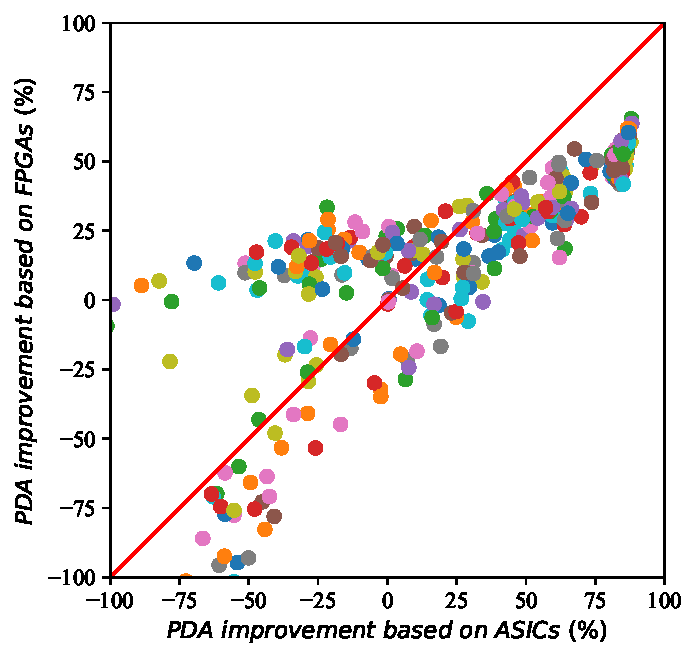
\includegraphics[width=0.7\linewidth]{./figs/AC-AM-AMG-Evo8_ASIC_FPGA.pdf}
    \caption{Evo8中的所有乘法器在ASIC和FPGA下的PDA提升}
    \label{AC:AM:AMG:Fig:Evo8_ASIC_FPGA.pdf}
\end{figure}

图\ref{AC:AM:AMG:Fig:Evo8_ASIC_FPGA.pdf}展示了不同乘法器在ASIC和FPGA下分别与对应的精确乘法器相比得到的PDA提升,
其中ASIC的结果是通过DC基于2GHz的时钟频率约束在开源的7nm工艺库\cite{ASAP7_github}上进行综合得到的,FPGA的结果是通过Vivado 2023.1在Virtex UltraScale+系列的器件xcvu3p-ffvc1517-3-e上基于100MHz时钟频率约束进行综合、布局布线得到的。
精确乘法器在DC和Vivado中分别通过DesignWare库\cite{IP:DesignWare}和Xilinx Multiplier LogiCORE IP\cite{IP:LogiCORE}自动构建,PDA提升由下式进行计算:
\begin{equation}
    \label{AC:AM:AMG:Eq:PDA_Imp}
    \frac{\text{PDA}_{ext} - \text{PDA}_{app}}{\text{PDA}_{ext}} *100
\end{equation}
其中$\text{PDA}_{app}$和$\text{PDA}_{ext}$分别代表近似乘法器和精确乘法器的PDA值,需要注意的是在FPGA中乘法器的面积指标由使用的LUT个数表示。
在图\ref{AC:AM:AMG:Fig:Evo8_ASIC_FPGA.pdf}中,每个点代表一个乘法器,横轴和纵轴分别代表在ASIC和FPGA下相比精确乘法器的PDA提升,由式\eqref{AC:AM:AMG:Eq:PDA_Imp}计算得到,落在红线上的点代表该乘法器在ASIC和FPGA下实现了相同程度的硬件性能提升,可以看到许多乘法器并不在红线上,这意味着这些针对ASIC设计的乘法器在由FPGA映射后无法获得类似的收益,甚至有一些在ASIC下PDA收益为-25\%的近似乘法器在FPGA上却改进了25\%。这是因为Evo8\cite{AC:AM:CGP_Evoapprox8b}中的乘法器均由2或3输入的逻辑门构成,在ASIC设计中,可以利用综合工具对这些门级电路进行细粒度的控制和优化。然而,FPGA使用可配置的LUT作为逻辑单元,拥有与逻辑门完全不同的特性。此外,在FPGA中,布线延迟约占关键路径延迟的50\%\cite{FPGA:Vaughn},虽然在通常情况下LUT数目越少布线越容易,延迟越低,但由于布局后电路拓扑结构的不同,面积相等的两个近似乘法器的布线延迟很可能差异较大,因此在设计FPGA近似乘法器时也应同时考虑布线资源的优化。

\section{研究内容与创新点}

本文提出并开源了一个面向FPGA领域的基于贝叶斯优化的自动化近似乘法器生成方法,该方法假设乘法器的部分积在生成后、累加前存在一次由半加器阵列进行的压缩操作,
针对半加器提出了4种简化方法,利用贝叶斯优化对半加器阵列进行搜索,之后保留压缩后累加过程中部分积的粗粒度加法,创新点如下:
\begin{itemize}
    \item 设计了一种能够生成任意位宽下乘法器的半加器阵列电路的方法,同时根据半加器的两个同权重的输入确定每个半加器的权重,该权重能够反映半加器对输出结果的重要性,以及半加器简化后引入的误差大小;
    \item 提出了4种简化方法来优化半加器的电路,根据期望的面积(LUT个数)减少比例和每个半加器的权重来决定半加器阵列中哪些半加器被优化,形成一个高质量的搜索空间;
    \item 基于详细设计地能够同时反映误差和硬件成本的目标函数,利用并行贝叶斯优化对半加器阵列的优化空间进行搜索,之后利用多位宽的加法对压缩后的部分积直接进行累加,保证这些加法能够被EDA工具(如Vivado)有效地识别,并映射到FPGA中的进位链上;
    \item 与国际前沿工作中的1167个乘法器相比,生成的乘法器能够形成帕累拖前沿,在硬件成本和误差的乘积上平均有28.70\%-38.47\%的提升。
\end{itemize}

\section{研究方法}

\subsection{半加器阵列}

\begin{figure}[!h]
    \begin{minipage}[t]{0.45\linewidth}
      \centering
      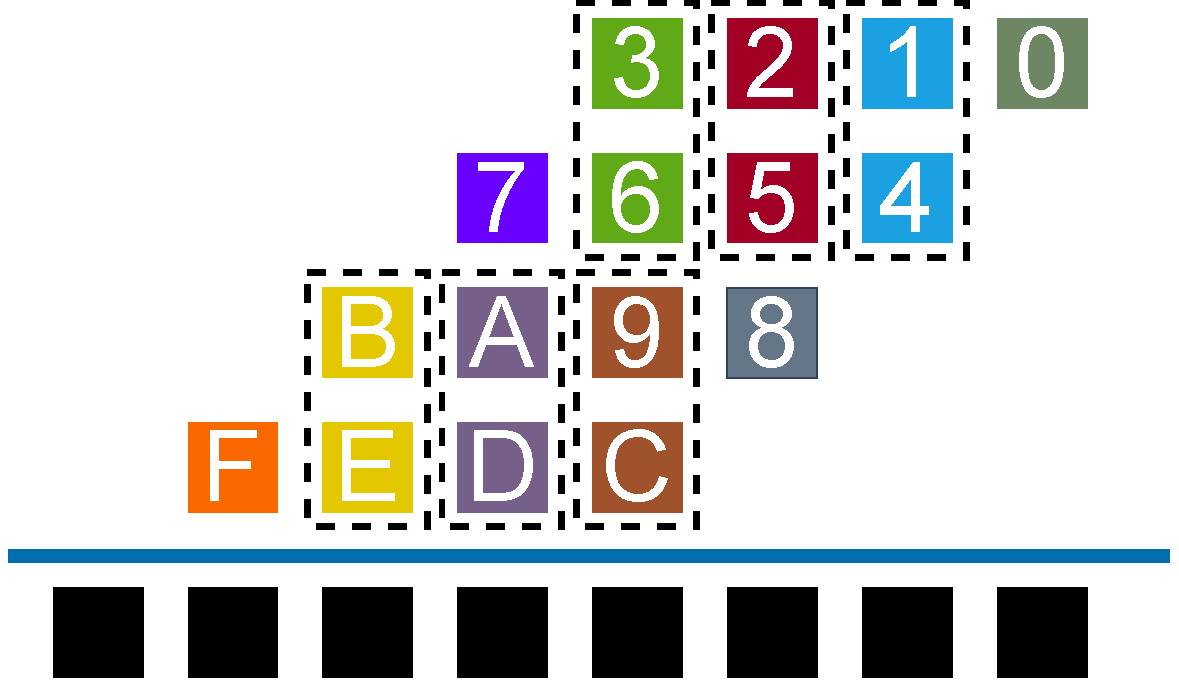
\includegraphics[width=\linewidth]{./figs/AC-AM-FPGA-AMG-4x4_orig.pdf}
      \caption{4$\times$4无符号乘法器的部分积阵列,共16个比特}
      \label{AC:AM:FPGA:AMG:Fig:4x4_orig}
    \end{minipage}
    \ \ \
    \begin{minipage}[t]{0.45\linewidth}
      \centering
      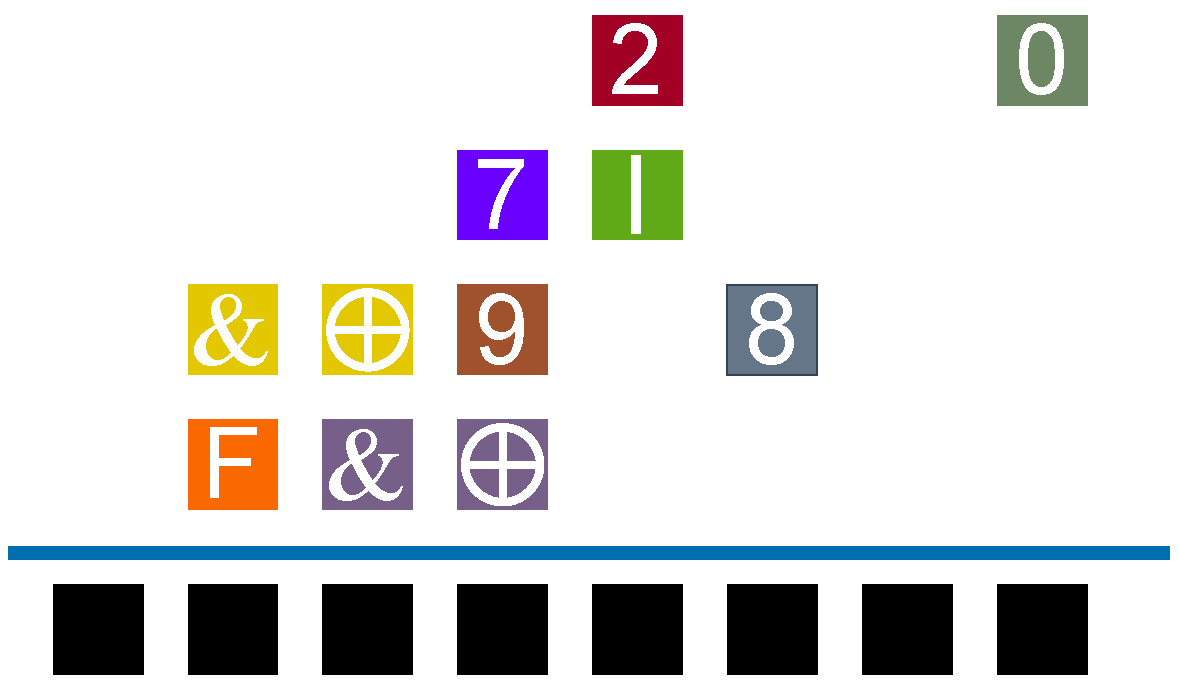
\includegraphics[width=\linewidth]{./figs/AC-AM-FPGA-AMG-4x4_compressed.pdf}
      \caption{利用搜索到的半加器阵列对部分积进行压缩后的结果}
      \label{AC:AM:FPGA:AMG:Fig:4x4_compressed}
    \end{minipage}
\end{figure}
图\ref{AC:AM:FPGA:AMG:Fig:4x4_orig}展示了一个由16个AND门生成的4$\times$4无符号乘法器的部分积阵列,以十六进制数进行标记。图中每个虚线框代表一个半加器,共6个半加器,组成一个半加器阵列对部分积进行压缩,阵列中每个半加器均对两个部分积比特进行运算,生成求和$Sum$与进位$Cout$。在图\ref{AC:AM:FPGA:AMG:Fig:4x4_orig}中,压缩后半加器阵列的输出和未被压缩的部分积比特0、7、8、F一起组成新的部分积阵列,对其进行累加求和后即能得到最终的运算结果。
若对半加器阵列进行优化,降低部分积阵列的规模,那么就可以减少后续累加电路的压力,有利于乘法器的硬件实现。
假设一个乘法器有$N$行部分积,每行部分积包含$M$个比特,则精确乘法器的半加器压缩阵列需要的半加器的数量$S$为:
\begin{equation}
    \label{AC:AM:FPGA:AMG:Eq:HA_number}
    S = (M-1) \times \lfloor \frac{N}{2} \rfloor
\end{equation}
其中$\lfloor \ \rfloor$表示向下取整。例如对图\ref{AC:AM:FPGA:AMG:Fig:4x4_orig}来说$S=6$。未被半加器阵列压缩的部分积个数为:
\begin{equation}
    \label{AC:AM:FPGA:AMG:Eq:Uncompress_number}
    N + (N \bmod 2) \times (M-1)
\end{equation}

\subsection{4种半加器的简化方法}

本文提出4种精确半加器的简化方法,其中3种能够有效降低半加器的硬件成本:
\begin{itemize}
    \item Eliminate: 直接删除该半加器,其求和$Sum$和进位输出$Cout$均接地;
    \item OR $Sum$: 求和输出$Sum$由半加器的两个输入进行或运算(OR)得到,进位输出$Cout$直接接地;
    \item Direct $Cout$: 将$Cout$连接到两个输入之一,并将$Sum$接地;
    \item Exact:保持该精确半加器的结构。
\end{itemize}

在上述的4种方法中,“Eliminate”和“OR $Sum$”会使半加器的结果变小,而“Direct $Cout$”会使半加器的结果变大,不同简化方法的结合能够降低半加器阵列的误差,提高乘法器的精度。对压缩阵列中的一部分半加器考虑简化,则生成高质量近似乘法器的问题变成了寻找较优简化操作组合的问题,可利用贝叶斯算法进行搜索。

\subsection{贝叶斯优化}

贝叶斯优化\cite{BBO:BayesianNeuralIPS}是一种基于顺序模型(Sequential model-based)的无梯度(Gradient-free)优化方法,常用于拟合评估昂贵的黑盒函数(Black-box function)。
在贝叶斯优化中,代理模型(Surrogate model,比如高斯过程Gaussian process)和获取函数(Acquisition function,比如预期改进expected improvement)一起用于对目标函数进行建模,并决定对哪个点进行采样以在下一次迭代中进行评估。贝叶斯优化需要已知点来训练代理模型,因此通常采用随机搜索的方法构建初始模型,每搜索并评估一个点后,算法对代理模型进行更新并通过最大化获取函数来生成下一个待评估的点。本文使用贝叶斯算法的变体TPE(Tree-structured Parzen estimator)\cite{BBO:TPE}来对优化空间进行搜索。

\subsection{误差分析}

由于部分积的权重不同,对不同的半加器进行简化会引入不同程度的误差,对每个半加器赋予一个权重,且大小与半加器两个输入比特的权重值一致,则图\ref{AC:AM:FPGA:AMG:Fig:4x4_orig}中输入为1、4和输入为B、E的两个半加器的权重分别为1和5。
理论上,由于不同半加器具有不同的权重值,贝叶斯算法在对压缩阵列进行优化时会倾向于简化低权重的半加器,保持高权重半加器的精确结构,以生成低误差高性能的近似乘法器。然而实际的贝叶斯优化算法无法做到如此高效,尤其是面对搜索空间是分离的而不是连续的情况,因此在搜索前可预先选择一部分半加器不参与优化,以提高生成的乘法器的精度。
假设乘法器的面积(即LUT个数)与压缩阵列中精确半加器的个数$S$成比例,并使用$R$来表示用户想要的与精确乘法器相比的面积百分比减少,则参与优化的半加器的数量为$\lfloor S \times R \rceil$,预先保留的精确半加器的数量为$S - \lfloor S \times R \rceil$,其中$\lfloor \ \rceil$表示四舍五入到最近的整数。
图\ref{AC:AM:FPGA:AMG:Fig:4x4_compressed}展示了$R=0.8$时利用搜索到的近似半加器阵列对原始部分积进行压缩后的结果,可以看到压缩后的新部分积阵列的比特总数为11,与图\ref{AC:AM:FPGA:AMG:Fig:4x4_orig}相比减少了31.25\%。另外需要注意的是,若压缩结果为图\ref{AC:AM:FPGA:AMG:Fig:4x4_compressed},则图\ref{AC:AM:FPGA:AMG:Fig:4x4_orig}中输入为B、E和A、D的两个半加器分别是预先保留的精确半加器和搜索得到的精确半加器。
压缩后的部分积和未被压缩的部分积一起组成新的部分积阵列,通过Verilog中的“+”操作符进行累加,可被FPGA的EDA工具高效地识别并映射到进位链,实现高性能的近似乘法器。

\subsection{目标函数}

贝叶斯优化需要一个目标函数(假设是$cost$)对每个点的好坏进行评估,$cost$越小的解质量越高,$cost$的计算方法决定了贝叶斯优化的搜索方向。例如,如果将$cost$设置为平均绝对误差MAE(即平均误差距离MED,见式\eqref{AC:Arith:MED}),那么贝叶斯优化将会忽略硬件成本开销,只着重于寻找MAE最小的乘法器,这会导致生成的乘法器性能很差。然而,近似乘法器的质量是由硬件成本和误差共同决定的,因此需要一个合适的$cost$定义方式。
乘法器的硬件成本可以由功耗延迟面积积PDA描述,而误差可以由MAE和均方误差MSE的乘积(Product of MAE and MSE, MM)表示,一个简单的同时考虑硬件开销和误差的$cost$计算方法是将其设置为PDA和MM的乘积。然而,根据分析,近似乘法器的MAE和MSE会随着PDA的降低指数级增长,这意味着若将$cost$设置为PDA$ \times $MM,则$cost$将由MM主导。为了能够使目标函数真实地反映出不同乘法器的质量,让具有较小$cost$的乘法器位于帕累拖前沿,将$cost$设置为PDAE,其定义为:
\begin{align}
    \text{PDAE} & = \text{PDA} \times \log_2 (\text{MM}^{\prime}) \label{AC:AM:FPGA:AMG:Eq:PDAE}  \\
    \text{MM}^{\prime} & = \text{MAE} \times \text{MSE} + 1 \label{AC:AM:FPGA:AMG:Eq:MM_prime}
\end{align}
根据式\eqref{AC:Arith:MED}、\eqref{AC:Arith:MSE}、式\eqref{AC:AM:FPGA:AMG:Eq:PDAE}、式\eqref{AC:AM:FPGA:AMG:Eq:MM_prime}可知精确乘法器的$cost=0$。


\subsection{优化流程}


\begin{figure}[!htbp]
    \centering
    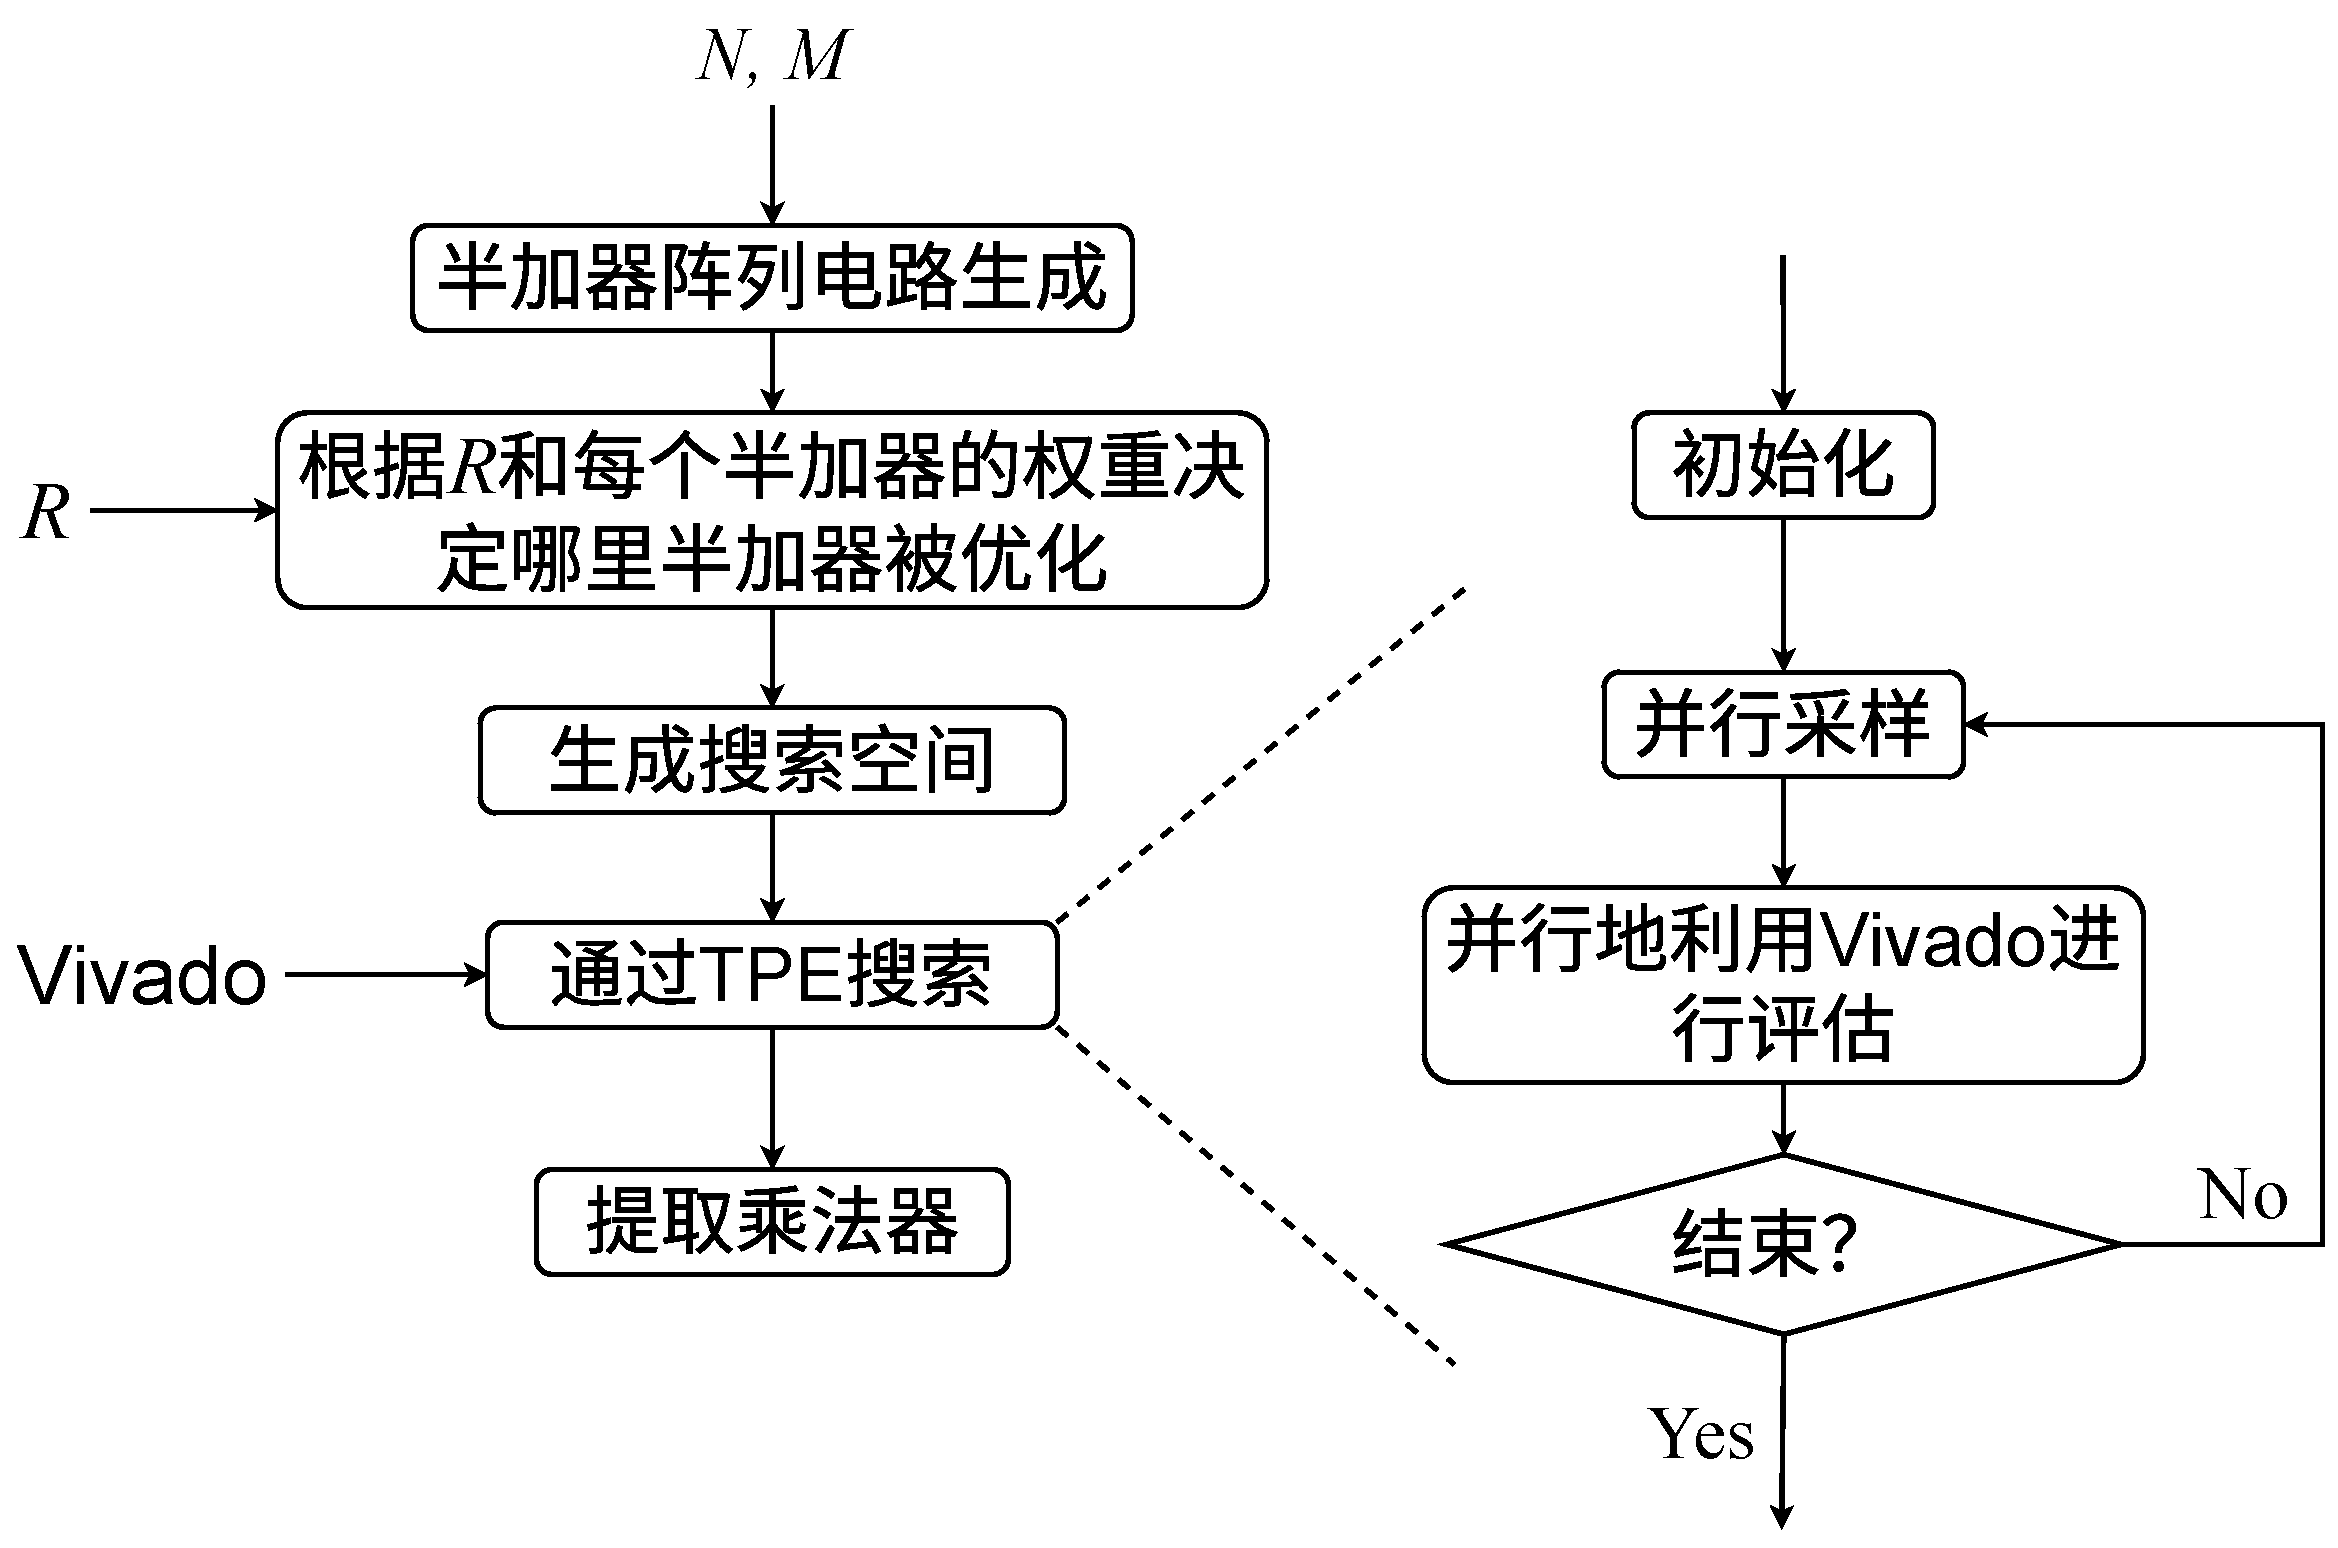
\includegraphics[width=0.8\linewidth]{./figs/AC-AM-FPGA-AMG-flow.pdf}
    \caption{整体流程}
    \label{AC:AM:FPGA:AMG:Fig:flow}
\end{figure}

图\ref{AC:AM:FPGA:AMG:Fig:flow}展示了整体的优化流程,首先根据乘法器的位宽$N$和$M$生成精确乘法器的半加器阵列电路并确定每个半加器的权重,接着根据用户想要的面积减少比例$R$和每个半加器的权重决定哪些半加器被优化,然后针对选定的半加器基于提出的4种简化方法生成优化空间,利用TPE并行地进行搜索,在搜索时直接利用Synopsys VCS和Vivado对生成的乘法器进行仿真、综合、布局、布线,得到$\text{MM}^{\prime}$和PDA,计算$cost$值。当程序达到规定的时间限制或最大迭代次数后中止,提取$cost$最小的多个乘法器与国际前沿工作进行对比。

\section{实验结果}

为了全面评估提出的自动化方法,考虑无符号8$\times$8乘法器并将$R$设置为多个值:$R \in \{ 0.3,\ 0.4,\ 0.5,\ 0.6,\ 0.7 \}$,对$R$的每个取值在60核Intel Xeon服务器上运行48小时之后提取每个$R$下$cost$较小的一批乘法器与已有的工作进行比较。
对比的乘法器除了\ref{ASIC实验结果}提到的众多ASIC近似乘法器之外,也包括一个FPGA近似乘法器库ApproxFPGAs\cite{AC:AM:FPGA:ApproxFPGAs}和通过手动修改LUT编码的方法生成的FPT22\cite{AC:AM:FPGA:FPT22}、CaCc\cite{AC:AM:FPGA:CaCc}、SMApproxLib\cite{AC:AM:FPGA:SMApproxLib}、TCAD22\cite{AC:AM:FPGA:TCAD22},总共1167个近似乘法器。同时,由Vivado采用Xilinx LogiCORE IP\cite{IP:LogiCORE}自动构建的和基于华莱士树结构实现的精确乘法器(分别被命名为Xilinx Default IP和Wallace)也被纳入比较范围。

所有的乘法器均通过Synopsys VCS S-2021.09-SP2和Vivado 2023.1基于Xilinx Virtex UltraScale+系列的器件xcvu3p-ffvc1517-3-e进行仿真、综合、布局布线,提取数据后计算MM$\prime$和PDA。

\begin{figure}[!htbp]
    \centering
    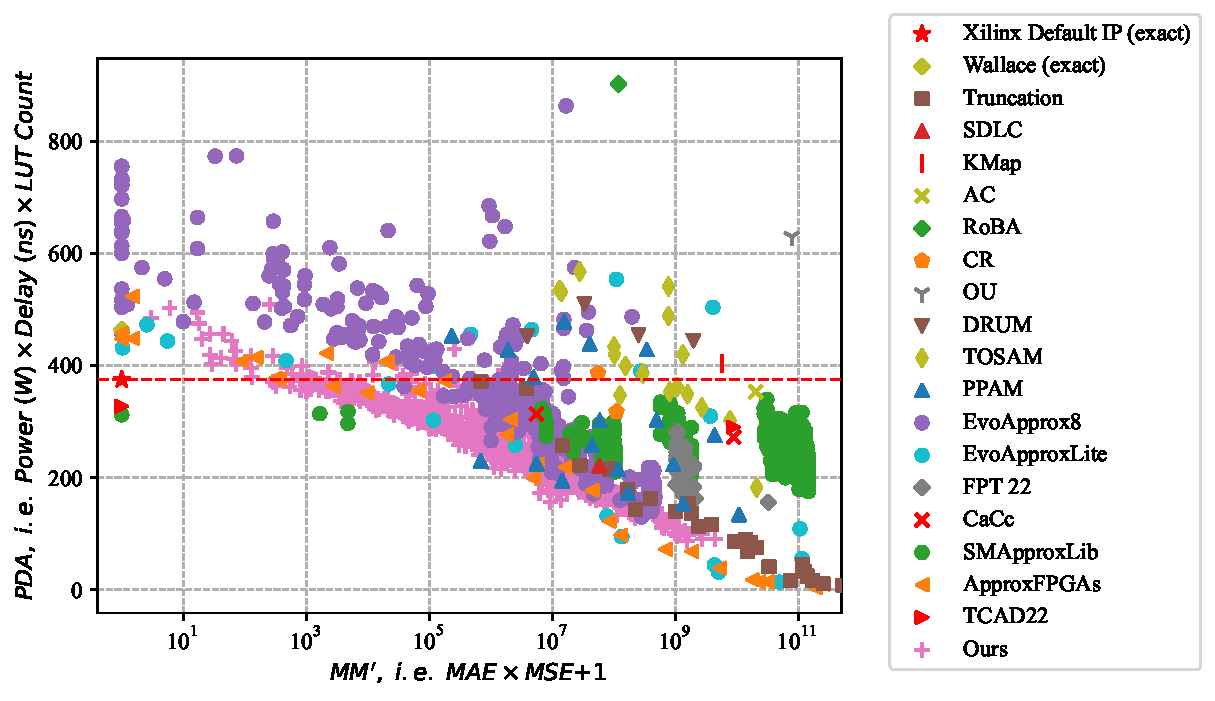
\includegraphics[width=\linewidth]{./figs/AC-AM-FPGA-AMG-PDA_MM_prime.pdf}
    \caption{不同乘法器的PDA和MM$^{\prime}$对比图}
    \label{AC:AM:FPGA:AMG:Fig:PDA_MM_prime}
\end{figure}

图\ref{AC:AM:FPGA:AMG:Fig:PDA_MM_prime}展示了不同乘法器的PDA和MM$\prime$散点图,可以看到基于本文生成的乘法器与别的乘法器一起组成了帕累拖前沿。SMApproxLib和TCAD22中有两个乘法器是精确乘法器,硬件开销比基于Xilinx LogiCORE IP实现的乘法器(图中的Xilinx Default IP)更低,具体来讲,这两个乘法器消耗的LUT资源比Xilinx Default IP少20\%左右,关键路径延迟增加了约5\%,这与文献\cite{AC:AM:FPGA:SMApproxLib}和文献\cite{AC:AM:FPGA:TCAD22}中描述地一致。
SMApproxLib中有三个近似乘法器以较小的误差(MM$^\prime\in[10^3,10^4]$)实现了较高的硬件性能。
同时,从图中可以看出,FPT22、CaCc、SMApproxLib和TCAD22这些基于LUT编码方法设计的近似乘法器之间误差相差较大,无法根据需求进行灵活地调整,应用场景较窄,尤其是SMApproxLib。
尽管EvoApprovx8b\cite{AC:AM:CGP_Evoapprox8b}是面向ASIC的,但基于自动化方法生成的近似乘法器之间具有较小的质量差异,能够为具有不同误差容忍度的应用程序提供更多选择。
从图中可以看出,当MM$^\prime \in [10^8,10^{11}]$时,EvoApproveLite\cite{AC:AM:CGP_EvoLite}和ApprovxFPGA\cite{AC:AM:FPGA:ApproxFPGAs}中的乘法器比其他乘法器的质量更高,但这些乘法器可能并不实用,因为它们要求应用具有较大的误差容忍度。
另外,图\ref{AC:AM:FPGA:AMG:Fig:PDA_MM_prime}中参与比较的近似乘法器是是从所有生成的乘法器中基于PDAE值选出的,可以看到具有小PDAE值的近似乘法器都处于帕累拖前沿,这证明了将目标函数$cost$定义为PDAE的合理性,即PDAE有效地指导了贝叶斯优化的搜索方向。

\begin{table*}[!htbp]
    \renewcommand{\arraystretch}{1.4}
    % \setlength\tabcolsep{3.76pt}
    \caption{根据MM$^\prime$对乘法器进行分组后对比每组最好的PDAE值}
    \begin{center}
    \scalebox{0.68}{
        \begin{tabular}{|c|c|c|c|c|c|c|c|c|}
        \hline
         & \multicolumn{2}{|c|}{\textbf{$\text{MM}^{\prime} \in [10^3,10^7] $}} & \multicolumn{2}{|c|}{\textbf{$\text{MM}^{\prime} \in [10^3,10^8] $}} & \multicolumn{2}{|c|}{\textbf{$\text{MM}^{\prime} \in [10^4,10^7] $}} & \multicolumn{2}{|c|}{\textbf{$\text{MM}^{\prime} \in [10^4,10^8] $}} \\
        \cline{1-9}
        \textbf{\textit{Group}} & \textbf{\textit{Best PDAE}} & \textbf{\textit{Imp. (\%)}} & \textbf{\textit{Best PDAE}} & \textbf{\textit{Imp. (\%)}} & \textbf{\textit{Best PDAE}} & \textbf{\textit{Imp. (\%)}} & \textbf{\textit{Best PDAE}} & \textbf{\textit{Imp. (\%)}}  \\
        \hline
        Truncation & 7205.03 & 50.90 & 5488.09 & 35.53 & 7205.03 & 49.60 & 5488.09 & 33.83 \\
        \hline
        SDLC \cite{AC:AM:SDLC} & \multirow{6}{*}{5709.04} & \multirow{6}{*}{38.03} & \multirow{6}{*}{5709.04} & \multirow{6}{*}{38.03} & \multirow{6}{*}{5709.04} & \multirow{6}{*}{36.39} & \multirow{6}{*}{5709.04} & \multirow{6}{*}{36.39} \\
        KMap \cite{AC:AM:KMap} & & & & & & & & \\
        AC \cite{AC:AM:AC} & & & & & & & & \\
        RoBA \cite{AC:AM:RoBA} & & & & & & & & \\
        CR \cite{AC:AM:CR} & & & & & & & & \\
        OU \cite{AC:AM:OU} & & & & & & & & \\
        \hline
        DRUM \cite{AC:AM:DRUM} & 9909.35 & 64.30 & 9909.35 & 64.30 & 9909.35 & 63.35 & 9909.35 & 63.35 \\
        \hline
        TOSAM \cite{AC:AM:TOSAM} & 6247.27 & 43.37 & 6247.27 & 43.37 & 6247.27 & 41.87 & 6247.27 & 41.87 \\
        \hline
        PPAM \cite{AC:AM:PPAM} & 4461.53 & 20.70 & 4461.53 & 20.70 & 4461.53 & 18.61 & 4461.53 & 18.61 \\
        \hline
        EvoApprox8b \cite{AC:AM:CGP_Evoapprox8b} & 4857.81 & 27.17 & 4340.22 & 18.48 & 4857.81 & 25.25 & 4340.22 & 16.33 \\
        \hline
        EvoApproxLite \cite{AC:AM:CGP_EvoLite} & 5088.03 & 30.46 & 3442.06 & -2.79 & 5088.03 & 28.63 & 3442.06 & -5.50 \\
        \hline
        FPT22 \cite{AC:AM:FPGA:FPT22} & 5010.96 & 29.40 & 5010.96 & 29.40 & 5010.96 & 27.53 & 5010.96 & 27.53 \\
        \hline
        CaCc \cite{AC:AM:FPGA:CaCc} & 7017.36 & 49.58 & 7017.36 & 49.58 & 7017.36 & 48.25 & 7017.36 & 48.25 \\
        \hline
        SMApproxLib \cite{AC:AM:FPGA:SMApproxLib} & 3356.49 & -5.41 & 3356.49 & -5.41 & 6266.03 & 42.05 & 5801.66 & 37.41 \\
        \hline
        ApproxFPGAs \cite{AC:AM:FPGA:ApproxFPGAs} & 4151.85 & 14.79 & 3220.87 & -9.85 & 4429.49 & 18.02 & 3220.87 & -12.74 \\
        \hline
        TCAD22 \cite{AC:AM:FPGA:TCAD22} & 9584.22 & 63.09 & 9584.22 & 63.09 & 9584.22 & 62.11 & 9584.22 & 62.11 \\
        \hline
        This thesis & 3537.97 & / & 3537.97 & / & 3631.35 & / & 3631.35 & / \\
        \hline
        Avg. Imp. & / & 35.53 & / & 28.70 & / & 38.47 & 30.62 & / \\
        \hline
        \end{tabular}
    }
        \label{AC:AM:FPGA:AMG:Table:PDAE}
        \end{center}
\end{table*}


为了更直观地比较不同近似乘法器的质量,将不同乘法器按照MM$^\prime$分组,并挑选出每组中最佳的PDAE值进行对比。
表\ref{AC:AM:FPGA:AMG:Table:PDAE}显示了分组后每组最好的PDAE值,按照本文的方法生成的近似乘法器的PDAE比别的组平均提高了28.70\%-38.47\%。
如果将MM$^\prime$限制在$[10^4,10^7]$的范围内,本文生成的乘法器在所有乘法器中效果最好。


\section{本章小结}

本章提出了一种面向FPGA的自动化近似乘法器设计方法,该方法假设乘法器的部分积在累加前存在一次由半加器阵列进行的压缩操作,利用贝叶斯算法基于提出的4种半加器简化方法对半加器阵列进行优化,保留压缩后累加过程中部分积的粗粒度加法,以使FPGA的EDA工具对其进行有效地识别,映射到进位链,提高电路性能。与国际前沿工作中的1167个近似乘法器相比,基于本文的方法生成的乘法器位于帕累拖前沿,综合指标比已有的乘法器平均提高了28.70\%-38.47\%。尽管实验是基于FPGA和均匀分布进行的,但该方法可以很容易地被拓展到ASIC领域和非均匀分布。
